\subsection{Evaluar fuera del periodo de ajuste}
\subsubsection*{Partición temporal y prueba sin reajuste}
Se mantienen las decisiones del 2.2: modelos de caudal con lluvia del mismo mes y del mes anterior, ajustados con 206 meses válidos hasta diciembre de 2016. Aquí se abren únicamente los 68 meses comunes de enero de 2017 a diciembre de 2022. No se vuelven a elegir modelos, rezagos, transformaciones ni parámetros a partir de esta prueba. Los años completos definen la partición cronológica, pero se excluyen pares inválidos: junio y julio de 2021 y marzo y abril de 2022. Junio de 2021 y marzo de 2022 carecen de datos mensuales completos; los meses siguientes pierden la lluvia antecedente CHIRPS. No hay mezcla aleatoria de ajuste y prueba ni relleno de huecos. Se usa precipitación original, no anomalías, por lo que no se calcula una nueva climatología de predictores con la reserva.
\subsubsection*{Ecuaciones congeladas y referencia}
Se aplican exactamente las ecuaciones de caudal del 2.2, con salida max(0, expresión): IMERG, -87,269198 + 0,465439 P(t) + 0,433065 P(t-1); CHIRPS, -35,852625 + 0,422155 P(t) + 0,434939 P(t-1). Q está en m$^3$/s y P en mm/mes. La referencia principal es la climatología mensual de Q estimada exclusivamente con los 206 meses de ajuste; también se muestra la media constante de ese ajuste. Se conserva una huella SHA-256 del archivo de parámetros para verificar que no cambió. Como P(t) se conoce al terminar el mes, esta prueba evalúa estimación mensual retrospectiva, no un pronóstico disponible antes de observar la lluvia del mes.
\subsubsection*{Resultados fuera del ajuste}
En los mismos 68 meses, CHIRPS obtiene RMSE 42,14 m$^3$/s, MAE 30,23, sesgo 2,47 y NSE 0,60; IMERG obtiene RMSE 43,77, MAE 34,49, sesgo -10,06 y NSE 0,57. El sesgo se define como estimado-observado: negativo indica subestimación. NSE=1-SSE/SST compara el error con la media del periodo evaluado; no sustituye la comparación explícita con la climatología entrenada. Esta última tiene RMSE 51,14. La reducción de RMSE frente a ella es 14,41 \% para IMERG y 17,61 \% para CHIRPS.
\begin{center}\small\begin{tabular}{lrrrrr}\hline
Fuente & n & RMSE & MAE & Sesgo & NSE \\ \hline
IMERG & 68 & 43,77 & 34,49 & -10,06 & 0,57 \\
CHIRPS & 68 & 42,14 & 30,23 & 2,47 & 0,60 \\
Media & 68 & 67,68 & 53,90 & -9,44 & -0,02 \\
Climatologia & 68 & 51,14 & 39,25 & -8,03 & 0,42 \\
\hline\end{tabular}\end{center}
\begin{figure}[H]\centering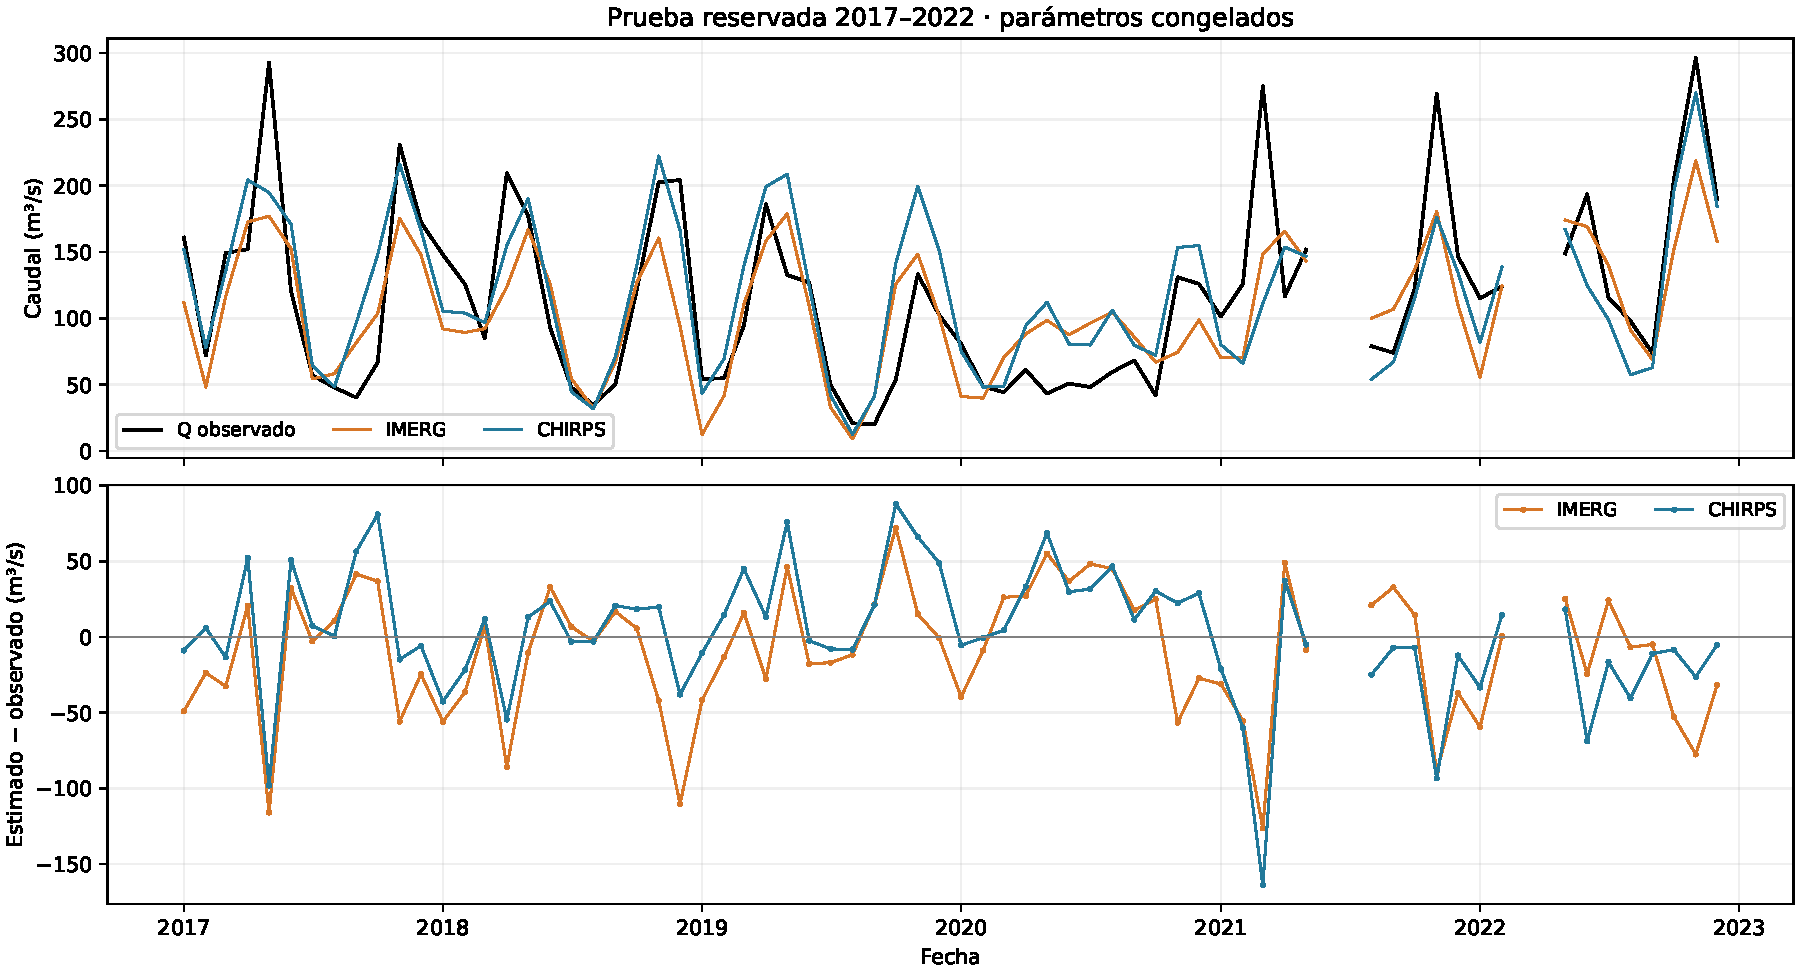
\includegraphics[width=\linewidth]{../apartado_2_3/reserva_series.pdf}\caption{Series y errores de los modelos congelados, 2017--2022.}\end{figure}
\subsubsection*{Estabilidad entre periodos y diferencia entre productos}
El orden de desempeño se invierte respecto del desarrollo: IMERG tenía RMSE 56,43 frente a 63,87 de CHIRPS; en la reserva CHIRPS es ligeramente mejor. La diferencia RMSE\_CHIRPS-RMSE\_IMERG es -1,63 m$^3$/s, pequeña frente al tamaño de los errores. La tabla anual permite examinar años favorables y desfavorables sin reajustar por año. Se calcula, además, un intervalo descriptivo de la diferencia mediante 3000 remuestreos pareados de bloques calendario de seis meses, manteniendo juntas las dos fuentes y preservando los huecos. Se repite con doce meses como sensibilidad; no se remuestrean meses aislados como si fueran independientes. Son intervalos aproximados con solo seis años, no una prueba de superioridad universal. El intervalo central del 95 \% con bloques de seis meses va de -7,76 a 5,89 m$^3$/s y con doce meses de -7,83 a 5,62; ambos incluyen cero. No hay evidencia sólida aquí de superioridad general de una fuente. CHIRPS tiene menor RMSE en 2017, 2018, 2020 y 2022; IMERG en 2019 y 2021. En 2020 el NSE es negativo para ambos (-0,59 y -0,17), lo que advierte estabilidad limitada respecto de la variabilidad de ese año, sin sustituir la referencia climatológica entrenada.
\begin{center}\small\begin{tabular}{lrrrrr}\hline
Fuente & Año & n & RMSE & MAE & Sesgo \\ \hline
IMERG & 2017 & 12 & 46,39 & 37,16 & -13,57 \\
IMERG & 2018 & 12 & 47,78 & 34,45 & -22,85 \\
IMERG & 2019 & 12 & 31,22 & 25,05 & 3,44 \\
IMERG & 2020 & 12 & 37,30 & 34,45 & 12,42 \\
IMERG & 2021 & 10 & 57,84 & 46,44 & -22,95 \\
IMERG & 2022 & 10 & 39,00 & 30,73 & -20,75 \\
CHIRPS & 2017 & 12 & 45,88 & 32,94 & 9,44 \\
CHIRPS & 2018 & 12 & 26,99 & 22,54 & -4,64 \\
CHIRPS & 2019 & 12 & 44,12 & 33,51 & 28,63 \\
CHIRPS & 2020 & 12 & 32,04 & 26,12 & 25,13 \\
CHIRPS & 2021 & 10 & 64,69 & 43,15 & -35,70 \\
CHIRPS & 2022 & 10 & 30,37 & 24,31 & -17,74 \\
Climatologia & 2017 & 12 & 52,57 & 36,85 & -22,10 \\
Climatologia & 2018 & 12 & 35,89 & 29,81 & -16,80 \\
Climatologia & 2019 & 12 & 38,79 & 36,16 & 22,30 \\
Climatologia & 2020 & 12 & 52,65 & 45,03 & 41,14 \\
Climatologia & 2021 & 10 & 60,98 & 38,53 & -33,12 \\
Climatologia & 2022 & 10 & 63,82 & 50,95 & -50,95 \\
\hline\end{tabular}\end{center}
\begin{center}\small\begin{tabular}{lrrr}\hline
Bloque (meses) & Diferencia RMSE & Percentil 2,5 & Percentil 97,5 \\ \hline
6 & -1,63 & -7,76 & 5,89 \\
12 & -1,63 & -7,83 & 5,62 \\
\hline\end{tabular}\end{center}
\subsubsection*{Residuos frente al tiempo, al estimado y al mes calendario}
Se presentan errores estimado-observado frente al tiempo y al valor estimado, además del sesgo y RMSE por mes calendario. Las curvas temporales conservan los huecos. La tabla mensual tiene solo cinco a seis observaciones por mes: las diferencias orientan la revisión, pero no justifican correcciones estacionales nuevas ajustadas con esta prueba. Se examina la correlación del error con el mes anterior usando el calendario completo, sin unir artificialmente meses separados por faltantes. Persistencia, dispersión cambiante y errores concentrados en ciertos meses limitan los modelos y evitan tratar una correlación global como garantía predictiva. IMERG subestima en enero, noviembre y diciembre (sesgos -46,14, -50,99 y -38,57 m$^3$/s); CHIRPS muestra sobreestimación marcada en octubre (+33,65) y subestimación en marzo (-23,16). Estos patrones no se corrigen después de mirar la reserva. La correlación del error con el mes anterior es 0,21 para IMERG y 0,18 para CHIRPS: la persistencia se reduce frente al desarrollo, pero no desaparece.
\begin{figure}[H]\centering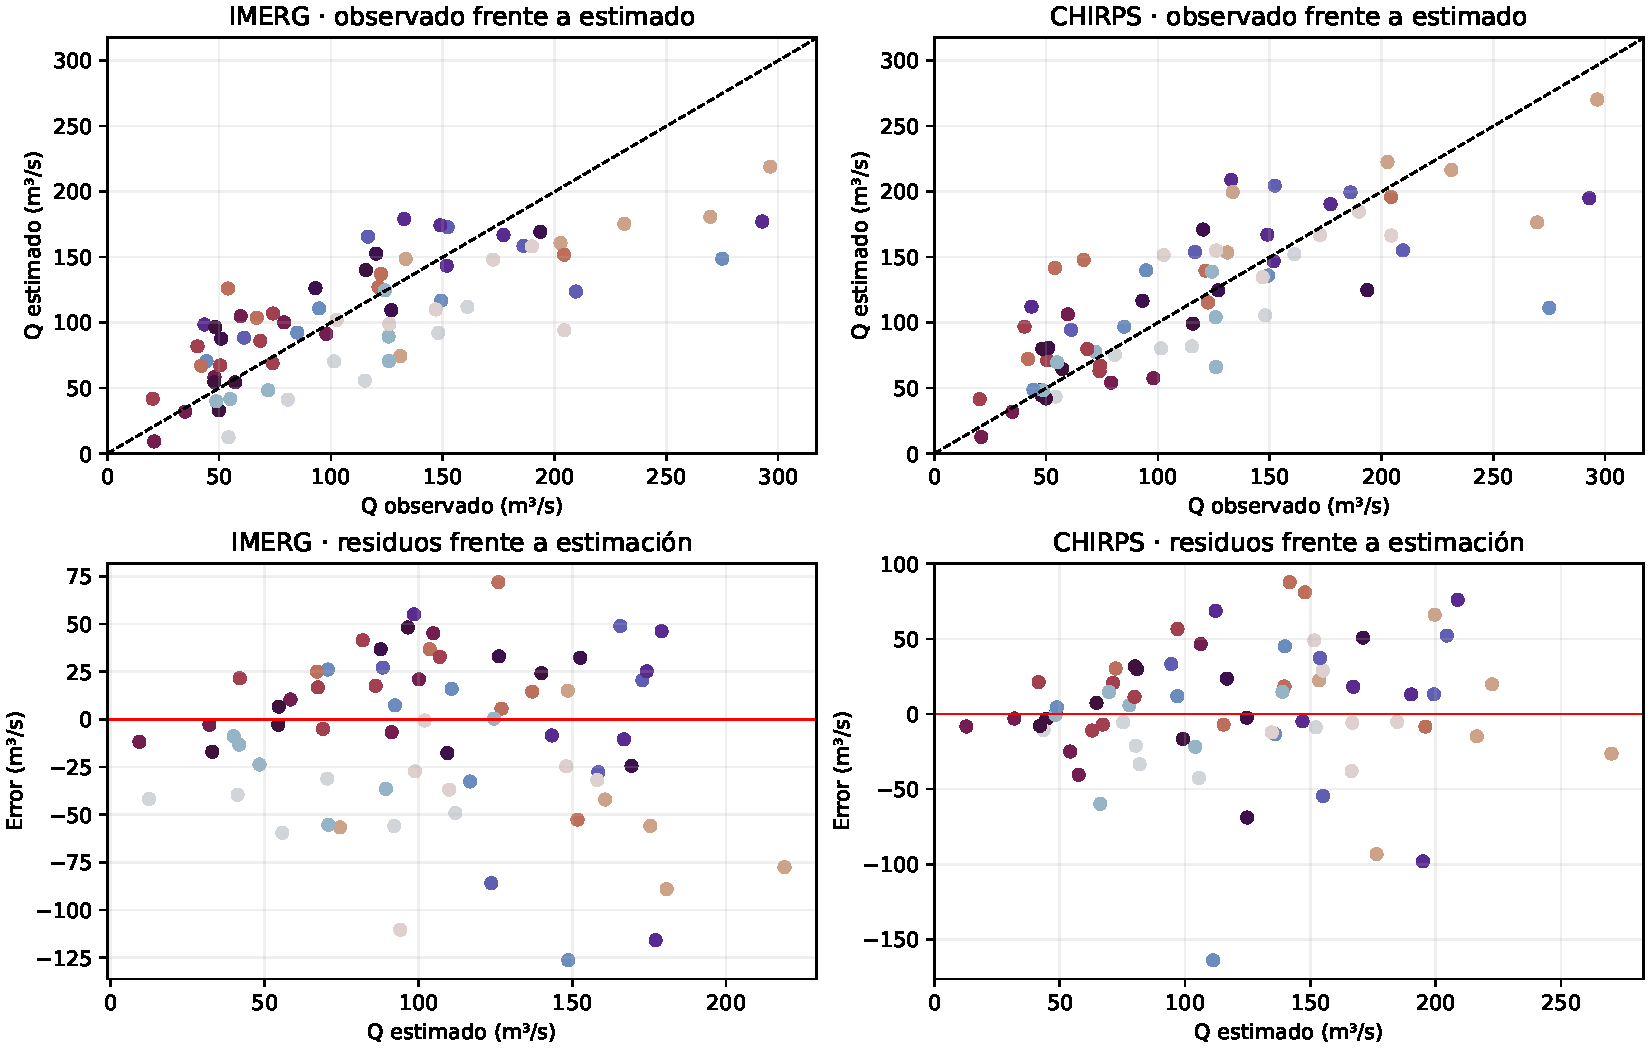
\includegraphics[width=\linewidth]{../apartado_2_3/reserva_dispersion_residuos.pdf}\caption{Predicciones y residuos frente al valor estimado.}\end{figure}
\begin{figure}[H]\centering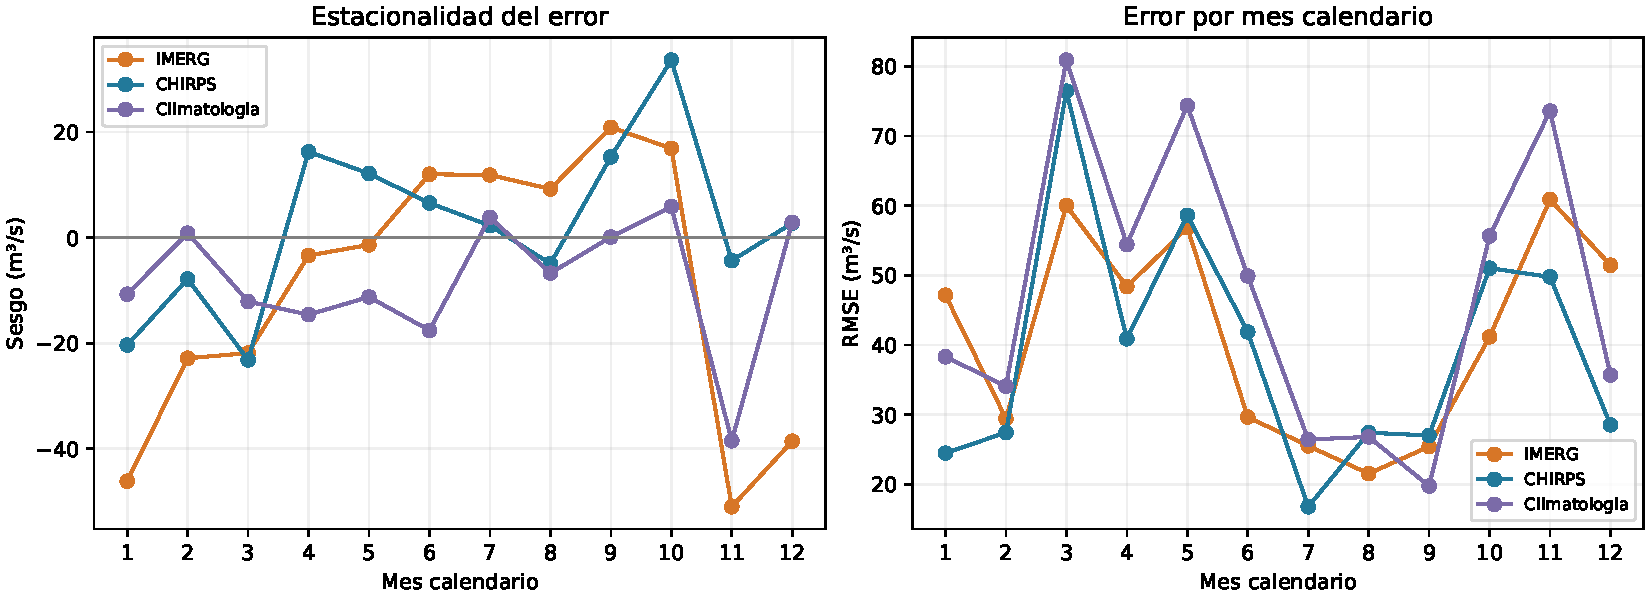
\includegraphics[width=\linewidth]{../apartado_2_3/reserva_meses.pdf}\caption{Estacionalidad residual y RMSE mensual en la reserva.}\end{figure}
\begin{center}\small\begin{tabular}{lrrrrr}\hline
Fuente & Mes & n & RMSE & MAE & Sesgo \\ \hline
IMERG & 1 & 6 & 47,16 & 46,14 & -46,14 \\
IMERG & 2 & 6 & 29,43 & 22,98 & -22,84 \\
IMERG & 3 & 5 & 60,02 & 41,69 & -21,86 \\
IMERG & 4 & 5 & 48,39 & 42,07 & -3,37 \\
IMERG & 5 & 6 & 56,86 & 43,52 & -1,37 \\
IMERG & 6 & 5 & 29,66 & 28,84 & 12,02 \\
IMERG & 7 & 5 & 25,52 & 19,79 & 11,88 \\
IMERG & 8 & 6 & 21,53 & 16,32 & 9,23 \\
IMERG & 9 & 6 & 25,43 & 22,54 & 20,89 \\
IMERG & 10 & 6 & 41,17 & 34,44 & 16,92 \\
IMERG & 11 & 6 & 60,89 & 56,01 & -50,99 \\
IMERG & 12 & 6 & 51,46 & 38,57 & -38,57 \\
CHIRPS & 1 & 6 & 24,47 & 20,35 & -20,35 \\
CHIRPS & 2 & 6 & 27,44 & 19,54 & -7,82 \\
CHIRPS & 3 & 5 & 76,44 & 47,75 & -23,16 \\
CHIRPS & 4 & 5 & 40,89 & 38,07 & 16,27 \\
CHIRPS & 5 & 6 & 58,62 & 46,46 & 12,15 \\
CHIRPS & 6 & 5 & 41,88 & 35,09 & 6,56 \\
CHIRPS & 7 & 5 & 16,77 & 13,35 & 2,29 \\
CHIRPS & 8 & 6 & 27,40 & 20,64 & -4,93 \\
CHIRPS & 9 & 6 & 27,02 & 21,32 & 15,31 \\
CHIRPS & 10 & 6 & 51,03 & 38,79 & 33,65 \\
CHIRPS & 11 & 6 & 49,78 & 40,45 & -4,35 \\
CHIRPS & 12 & 6 & 28,53 & 23,20 & 2,75 \\
\hline\end{tabular}\end{center}
\begin{center}\small\begin{tabular}{lrr}\hline
Fuente & r error antecedente & Fracción subestimada \\ \hline
IMERG & 0,21 & 0,56 \\
CHIRPS & 0,18 & 0,50 \\
\hline\end{tabular}\end{center}
\subsubsection*{Caudales altos, plausibilidad física y extrapolación}
Para definir caudal alto se usa el percentil 75 del ajuste, 141,54 m$^3$/s, sin elegir el umbral con la prueba. Se reportan por separado n, sesgo, MAE y RMSE de esa condición y del resto. En el grupo alto, el menor RMSE corresponde a CHIRPS (54,06 m$^3$/s), lo que debe leerse junto con los sesgos y la muestra. Se cuentan salidas negativas antes de aplicar el truncamiento a cero y entradas P(t) o P(t-1) fuera de los rangos del ajuste. El truncamiento asegura no negatividad, pero no conserva masa ni valida magnitudes extremas. No se aplica recorte superior, interpolación ni corrección posterior del sesgo. Cambios de almacenamiento, evapotranspiración, extracción y operación quedan fuera de estas regresiones. Los dos modelos subestiman caudales altos: sesgo -48,16 m$^3$/s para IMERG y -25,85 para CHIRPS, con 21 meses en el grupo. En los 47 meses bajos-medios, IMERG tiene menor RMSE (31,83 frente a 35,54). No hubo salidas brutas negativas en la reserva. CHIRPS presenta dos meses con predictores fuera del rango de ajuste, octubre y noviembre de 2022; IMERG ninguno. No se descartan esos meses para favorecer un resultado.
\textbf{Q alto (umbral de ajuste).}\begin{center}\small\begin{tabular}{lrrrr}\hline
Fuente & n & RMSE & MAE & Sesgo \\ \hline
IMERG & 21 & 62,74 & 52,52 & -48,16 \\
CHIRPS & 21 & 54,06 & 36,93 & -25,85 \\
Media & 21 & 102,94 & 91,20 & -91,20 \\
Climatologia & 21 & 73,94 & 59,13 & -57,89 \\
\hline\end{tabular}\end{center}
\textbf{Q bajo-medio.}\begin{center}\small\begin{tabular}{lrrrr}\hline
Fuente & n & RMSE & MAE & Sesgo \\ \hline
IMERG & 47 & 31,83 & 26,43 & 6,97 \\
CHIRPS & 47 & 35,54 & 27,24 & 15,13 \\
Media & 47 & 43,50 & 37,24 & 27,08 \\
Climatologia & 47 & 36,62 & 30,37 & 14,24 \\
\hline\end{tabular}\end{center}
\begin{center}\small\begin{tabular}{lrrrr}\hline
Fuente & Mín. bruto & Máx. bruto & Negativos & Fuera rango P \\ \hline
IMERG & 9,32 & 218,97 & 0 & 0 \\
CHIRPS & 12,76 & 270,15 & 0 & 2 \\
\hline\end{tabular}\end{center}
\subsubsection*{Lluvia local: no existe una reserva independiente adicional}
Los catorce meses completos de Zaragoza ya se utilizaron en el desarrollo y en el reajuste local del 2.2; no hay meses locales adicionales para evaluar honestamente esas ecuaciones congeladas. Por eso no se reutilizan como una nueva prueba final. Se conserva, solo como diagnóstico previo ya examinado en 2.2, el corte de siete meses de 2018 para ajustar y siete de 2019 para comprobar. En esa tabla se añade la referencia solicitada: precipitación del producto sin corrección para estimar lluvia local; IMERG es la referencia de la guía y CHIRPS su comparación paralela. Ese diagnóstico también participó en las decisiones del desarrollo y no equivale a una validación final independiente. Para cerrar esa parte se necesitan registros locales nuevos o previamente separados, que no se usen para calibrar ni elegir el modelo.
\begin{center}\small\begin{tabular}{lrrrrr}\hline
Fuente & Caso previo & n & RMSE & MAE & Sesgo \\ \hline
IMERG & Sin corrección & 7 & 108,19 & 95,51 & 95,51 \\
IMERG & Recta: diagnóstico previo & 7 & 41,85 & 36,76 & -17,40 \\
CHIRPS & Sin corrección & 7 & 85,28 & 67,75 & 67,75 \\
CHIRPS & Recta: diagnóstico previo & 7 & 30,50 & 25,58 & -14,29 \\
\hline\end{tabular}\end{center}
\subsubsection*{Fuentes compartidas y alcance de la independencia}
La separación temporal evita usar el caudal de prueba para ajustar la regresión, pero no garantiza independencia entre productos de precipitación y estaciones. IMERG Final combina información satelital con análisis de pluviómetros; CHIRPS combina información satelital y estaciones. No se ha verificado si Zaragoza integra las redes de ajuste de estos productos. Tampoco se presenta Q como un balance de agua cerrado ni como una medida causal de la lluvia. Fuentes metodológicas: NASA, IMERG (\url{https://gpm.nasa.gov/data/imerg}); Climate Hazards Center, CHIRPS (\url{https://chc.ucsb.edu/data/chirps}). El periodo reservado no se usó para ajustar ni seleccionar los modelos del 2.2, aunque sus series ya aparecieron en la exploración de 1.1 y 2.1. Se trata de una evaluación temporal fuera del ajuste, no de un experimento completamente ciego. Una comprobación prospectiva con años nuevos reforzaría la evidencia.
\subsubsection*{Conclusión del 2.3}
Existe una relación aprovechable para estimar caudal mensual a partir de lluvia contemporánea y antecedente: ambas fuentes mejoran la climatología en la prueba reservada. CHIRPS tiene el menor RMSE y MAE globales y un sesgo más cercano a cero en 2017--2022; la ventaja es pequeña y debe contrastarse con años, meses y condiciones de caudal, sin declarar un ganador general. Los modelos siguen siendo herramientas estadísticas retrospectivas de la misma cuenca, con limitaciones en extremos, estabilidad y causalidad. No se recomienda usarlos como pronósticos de crecidas ni extrapolarlos a otras cuencas. Para lluvia local, la utilidad continúa siendo exploratoria: no hay una prueba independiente adicional disponible.
